\section{Data and Monte Carlo Samples}
\label{sec:DataAndMC}

The data sample we use in this measurement was recorded by the CMS experiment in~2012 in LHC $pp$ collisions at $\sqrt{s}=$8~TeV. Integrated luminosity of the dataset is $L=$19.6~fb$^{-1}$. To select $W\gamma$ events, we use data collected by single muon and single electron triggers. The single muon trigger requires that in each event there is at least one reconstructed isolated muon with $P_T^{\mu}>$24~GeV and $|\eta|<$2.1. The isolation requirement imposes a restriction on the total energy of particles observed in a narrow cone around the muon. The single electron trigger requires at least one reconstructed electron with $P_T^{e}>$27~GeV that also passes a certain set of identification requirements, including isolation. Such trigger choice maximizes our chances to select $W\gamma$ events in $pp$ collisions that produce mostly less interesting and much more probable events of other types, such as multijets events.

In addition to the $W\gamma$-selected data sample, we also prepare the $Z\gamma$-selected data sample which is used for the background estimation (Ch.~\ref{sec:BackgroundSubtraction}) and cross checks (App.~\ref{sec:ZgCheck}). To select $Z\gamma$ events, we use double muon and double electron triggers. The double muon trigger requires a presence of at least two reconstructed muons with $P_T^{\mu}>$17~GeV and $P_T^{\mu}>$8~GeV per event. The double electron trigger requires a presence of at least two reconstructed electrons with $P_T^{e}>$17~GeV and $P_T^{e}>$8~GeV that also satisfy several quality criteria.

The simulated samples (often called ``Monte Carlo'' or ``MC'' samples) used in this measurement are produced centrally by the CMS simulation team. Information regarding MC samples used for our measurement is given in Tab.~\ref{tab:mc_bkg_samples} alongside with the corresponding cross sections at~8~TeV. All cross sections are calculated with kinematic restrictions matching to the kinematic restrictions of the samples. The kinematic restrictions for different samples differ and reflect theoretical divergencies for specific processes and detector acceptance. In all cases, however, the phase space of the sample is wider than the phase space probed in this measurement.

\begin{table}[h]
  \small
  \begin{center}
    \caption{Summary of simulated samples used in the measurement.}
    \begin{tabular}{|l|l|l|}
      \hline
      Process                              & Type & $\sigma$, pb  \\ \hline
      $W\gamma \rightarrow l\nu\gamma$     & signal & 554   \\ \hline %(NLO MCFM)
      $W$+jets$ \rightarrow l\nu $+jets   & background & 36257  \\ \hline %(NNLO FEWZ)
      DY+jets$ \rightarrow ll $+jets     & background & 3504  \\ \hline %(NNLO FEWZ)
      $t\bar{t}$+jets$\rightarrow 1l$+X    & background & 99    \\ \hline %(NNLO)
      $t\bar{t}$+jets$\rightarrow 2l$+X    & background & 24    \\ \hline
%      $t\bar{t}\gamma$                     & background & 1    \\ \hline
      $Z\gamma \rightarrow ll\gamma$       & background & 172   \\ \hline
    \end{tabular}
    \label{tab:mc_bkg_samples}
  \end{center}
\end{table} 

When we apply $W\gamma$ selection criteria to the data sample, selected events contain not only the events originating from the signal process but also events from other, background, processes. Tab.~\ref{tab:mc_bkg_samples} contains all sources that significantly contribute to the selected sample. $W\gamma \rightarrow l\nu\gamma$ contains $W\gamma \rightarrow \mu\nu\gamma$ and $W\gamma \rightarrow e\nu\gamma$ which are our signal samples and $W\gamma \rightarrow \tau\nu\gamma$ which is a background for both channels. The other samples listed in Tab.~\ref{tab:mc_bkg_samples} are background samples. They are used for the background estimation and cross checks as explained in detail in the remainder of the chapter. 

All MC samples were generated with MadGraph~5~\cite{ref_MadGraph} interfaced with PYHTIA~6~\cite{ref_Pythia}. The CTEQ6L1 PDF set was used~\cite{ref_CTEQ6L1}. The passage of the generated particles through the CMS detector is simulated with GEANT~4~\cite{ref_Geant4}. 

Cross section values corresponding to all genetated samples in Tab.~\ref{tab:mc_bkg_samples} are calculated by MCFM~\cite{ref_MCFM} or FEWZ~\cite{ref_FEWZ} except for the $Z\gamma$ sample. The uncertainty on normalization of the $Z\gamma$ sample gives a significant contribution to the uncertainty of the measurement because $Z\gamma$ MC sample is used to estimate the most significant background (Ch.~\ref{sec:BackgroundSubtraction_jtog}). MCFM provides a value of the cross section with uncertainty of~20\%. To decrease the uncertainty, we use a cross section of $Z\gamma$ measured at~8~TeV by CMS~\cite{ref_Zg8TeV} and recalculated for the phase space of the generated $Z\gamma$ MC sample. The recalculation procedure is described below.

% MATCHED AN TO THESIS
The $Z\gamma$ cross section of $\sigma=$2073$\pm$95$\pm$11$\pm$53~fb has been reported in the phase space described in~\cite{ref_Zg8TeV}. To determine the measured cross section  $\sigma_{ps1}$ in the phase space of the $Z\gamma$ MC sample, the following formula was used:
\begin{equation}
\sigma_{ps1} = \sigma_{ps2}^{meas.} \cdot \frac{N_{ps1}^{MC}}{N_{ps2}^{MC}},
\end{equation}
\noindent{where $\sigma_{ps2}^{meas.}$ is the~8~TeV cross section measured by CMS, $N_{ps1}^{MC}$ and $N_{ps2}^{MC}$ are numbers of events in the full phase space of $Z\gamma$ MC samples and in the phase space corresponding to the measured cross section  $\sigma_{ps2}^{meas.}$. The resulting $Z\gamma$ cross section is found to be $\sigma_{ps1}=$172~pb. }

%The NLO cross section of $W\gamma$ was calculated with the MCFM in the same phase space for which the $W\gamma$ sample was generated. The NNLO contribution is estimated to be~19\%-26\% of the NLO value~\cite{ref_theory_NNLO}. We use an NLO cross section value, and the NNLO estimate is used as an systematic uncertainty of the normalization of the $W\gamma$ sample when it is applicable. 

Inclusive simulated samples $W$+jets and DY+jets naturally contain events with the $W\gamma$ and $Z\gamma$ processes, and we explicitly exclude $W\gamma$ events from the $W$+jets sample and $Z\gamma$ events from the DY+jets samples. DY+jets, or DY, is a notation for the Drell Yan process, $pp\rightarrow\Z/\gamma\rightarrow ll$. The requirement on the invariant mass of the final state lepton pair in the DY+jets sample is $M_{ll}>$50~GeV. 

%WGToLNuG_TuneZ2star_8TeV-madgraph-tauola NLO MCFN
%WJetsToLNu_TuneZ2Star_8TeV-madgraph-tarball NLO FEWG
%DYJetsToLL_M-50_TuneZ2Star_8TeV-madgraph-tarball NLO FEWG
%TTJets_SemiLeptMGDecays_8TeV-madgraph
%TTJets_FullLeptMGDecays_8TeV-madgraph
%ZGToLLG_8TeV-madgraph

%https://twiki.cern.ch/twiki/pub/Main/WJetsCrossSectionMeasurementOutline8TeV/AN2014_114_v7.pdf
%https://arxiv.org/pdf/1610.04222.pdf
%(WJets note; has DYjets and Wjets samples and paper) 

All MC samples are normalized to the luminosity of the dataset $L_{DATA}=$19.6~pb$^{-1}$. To perform the normalization, weights of
\begin{equation}
  w = \frac{L_{DATA}}{L_{MC}} = \frac{L_{DATA} \sigma_{MC}}{N_{MC}}
\end{equation}
\noindent{are applied to each event in each MC sample, where $N_{MC}$ is the number of events in a given MC sample, and $\sigma_{MC}$ is a cross section of the process of MC sample within the phase space of the MC sample. Such weighted MC samples are used for various MC predictions mentioned in later sections and for all plots involving MC.}

At the instantaneous luminosities of LHC in~2012, as a rule, multiple $pp$ interactions occurred per bunch crossing. Multiple interactions are also simulated in the MC samples. However, MC samples are usually produced before data collection is finished, and have to be reweighted so that the distribution of the number of interactions (pileup or PU) in a simulated sample matches the data. The PU weights are assigned to each event in each MC sample to make the PU distribution in MC accurately describe PU in data.

To validate the procedure of the PU reweighting, we confirm that the agreement between data and MC in the distribution of the number of $pp$ interaction vertices in $Z\gamma\rightarrow\mu\mu\gamma$-selected datasets is good (Fig.~\ref{fig:DATAvsMC_nVtx}). We choose the $Z\gamma$ selected dataset instead of the $W\gamma$-selected dataset because the sample composition for $Z\gamma$ selection is understood better and normalizations of the MC samples that pass $Z\gamma$ selection are known better. The $Z\gamma$ selection is explained in Ch.~\ref{sec:AN_Selection} alongside with the $W\gamma$ selection.

\begin{figure}[htb]
  \begin{center}
   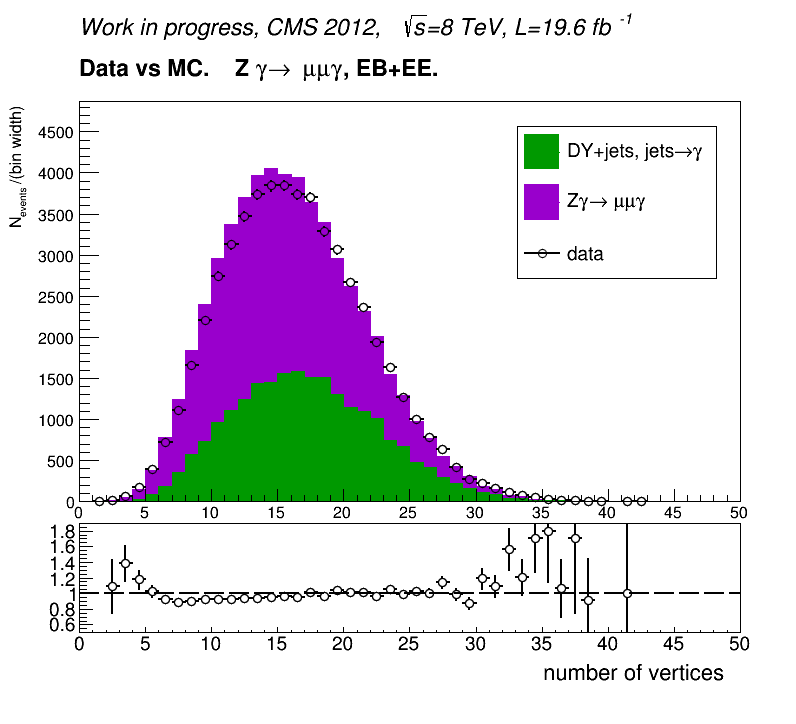
\includegraphics[width=0.45\textwidth]{../figs/figs_v11/MUON_ZGamma/PrepareYields/c_TotalDATAvsMC_EtaCommon__nVtx_noPU.png}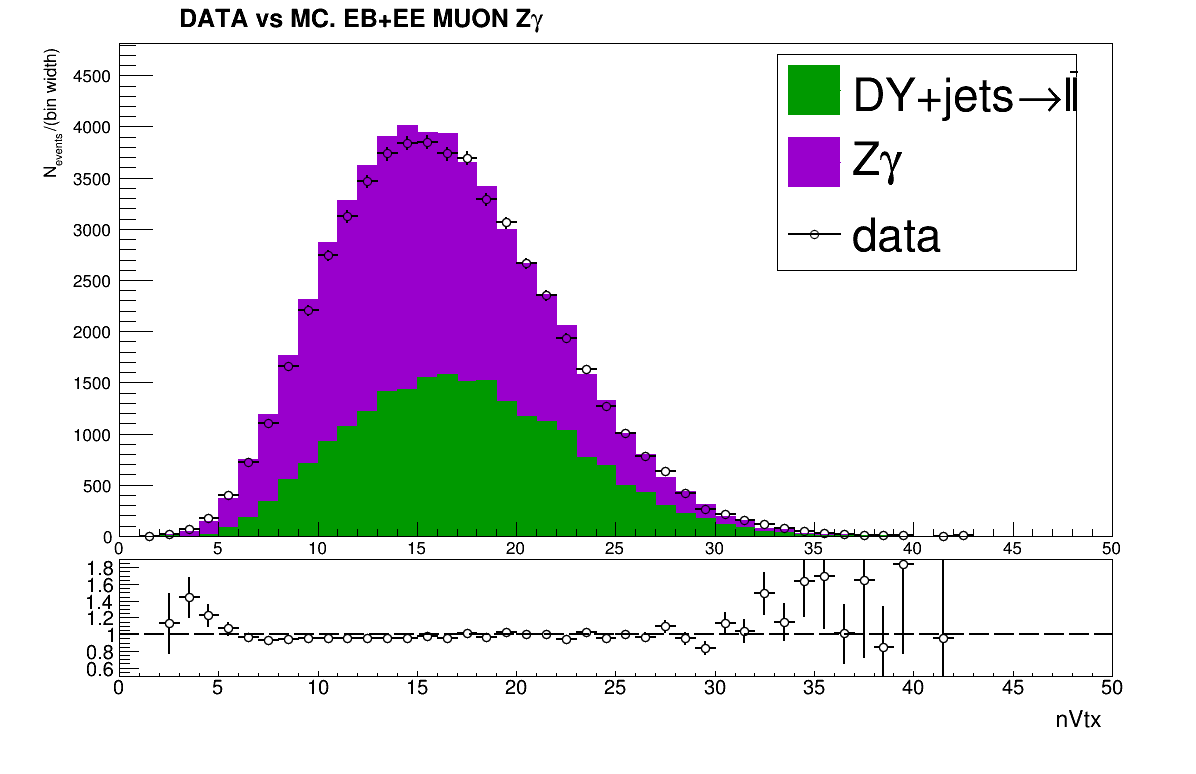
\includegraphics[width=0.45\textwidth]{../figs/figs_v11/MUON_ZGamma/PrepareYields/c_TotalDATAvsMC_EtaCommon__nVtx.png}
  \caption{Number of $pp$ interaction vertices of $Z\gamma$ candidates in the muon channel. Data vs MC. Left: no PU reweighting applied, right: PU reweighting applied. Ratio plot in the bottom shows data yields divided by total MC yields. EB+EE means that events with a final state photon reconstructed in the ECal barrel as well as  events with a final state photon reconstructed in the ECal endcap are shown on the plots.}
  \label{fig:DATAvsMC_nVtx}
  \end{center}
\end{figure}
